\documentclass{standalone}
\usepackage{tikz}
\usetikzlibrary{patterns,decorations.pathmorphing}
\tikzset{snake it/.style={decorate, decoration=snake}}
\begin{document}
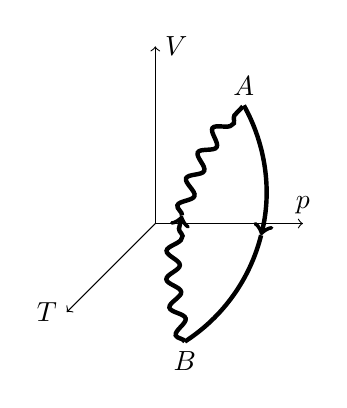
\begin{tikzpicture}[scale=1.5]
    \draw[->](0.25,0)--(1.5,0)node[above]{$p$};
    \draw[->](0.25,0)--(0.25,1.5)node[right]{$V$};
    \draw[->](0.25,0)--(-0.5,-0.75)node[left]{$T$};    
    \node[above]at(1,1){$A$};
    \node[below]at(0.5,-1){$B$};

    \draw[->,ultra thick](1,1)arc(29.169:-14.0295:1.505);
    \draw[-, ultra thick](1.146,-0.099)arc(-14.0295:-57.228:1.505);
    \draw[->,ultra thick, snake it](0.5,-1)arc(196.547:165.9635:2.025);
    \draw[-, ultra thick, snake it](0.476,0.068)arc(165.9635:135.680:2.025);
\end{tikzpicture}
\end{document}